\section{Purpose}
The Bloch equations provide a mathematical framework for characterizing the evolution of the magnetization over time. These equations describe the magnetization $B=(M_x, M_y, M_z)$ in terms of time $t$, the relaxation time $T_1$, $T_2$, and the external magnetic field $B$ and can be solved analytically with an explicitly defined pulse sequence. Though the Bloch equations play a crucial role in various applications of magnetic resonance imaging (MRI) and allow us to understand the behavior of the magnetization and obtain images, due to the nonlinear dynamics system they described, it is difficult to utilize the extensive parameters space in the pulse sequence to optimize our signal, especially when considering some physiological or technical limitations.
\\\\
Reinforcement Learning shows its huge potential in dealing with dynamic environments, particularly in areas such as gaming and autonomous systems (Chess and Go). It is a type of machine learning where an agent learns to make decisions by performing actions in an environment to maximize a reward signal. This approach allows the agent to learn from experience, adjusting its behavior over time to achieve the best results without knowing much about the action which have been used but simple rules.
\\\\
The main objective of this project is to optimizing MRI pulse sequence using Reinforcement Learning. Given a typical gradient-echo sequence-based signal, the goal is to design a new sequence that can produce an optimized signal under certain constraints including slew rate of a magnetization gradient field.

\section{Literature Review}
\textbf{Design pulse sequence by optimal control.}
\\\\
\textbf{Design pulse sequence by Reinforcement Learning.}

\section{Methodology}

\textbf{Reinforcement Learning: key concepts: agent, actions, environment, rewards.}

\begin{figure}[ht]
    \centering
    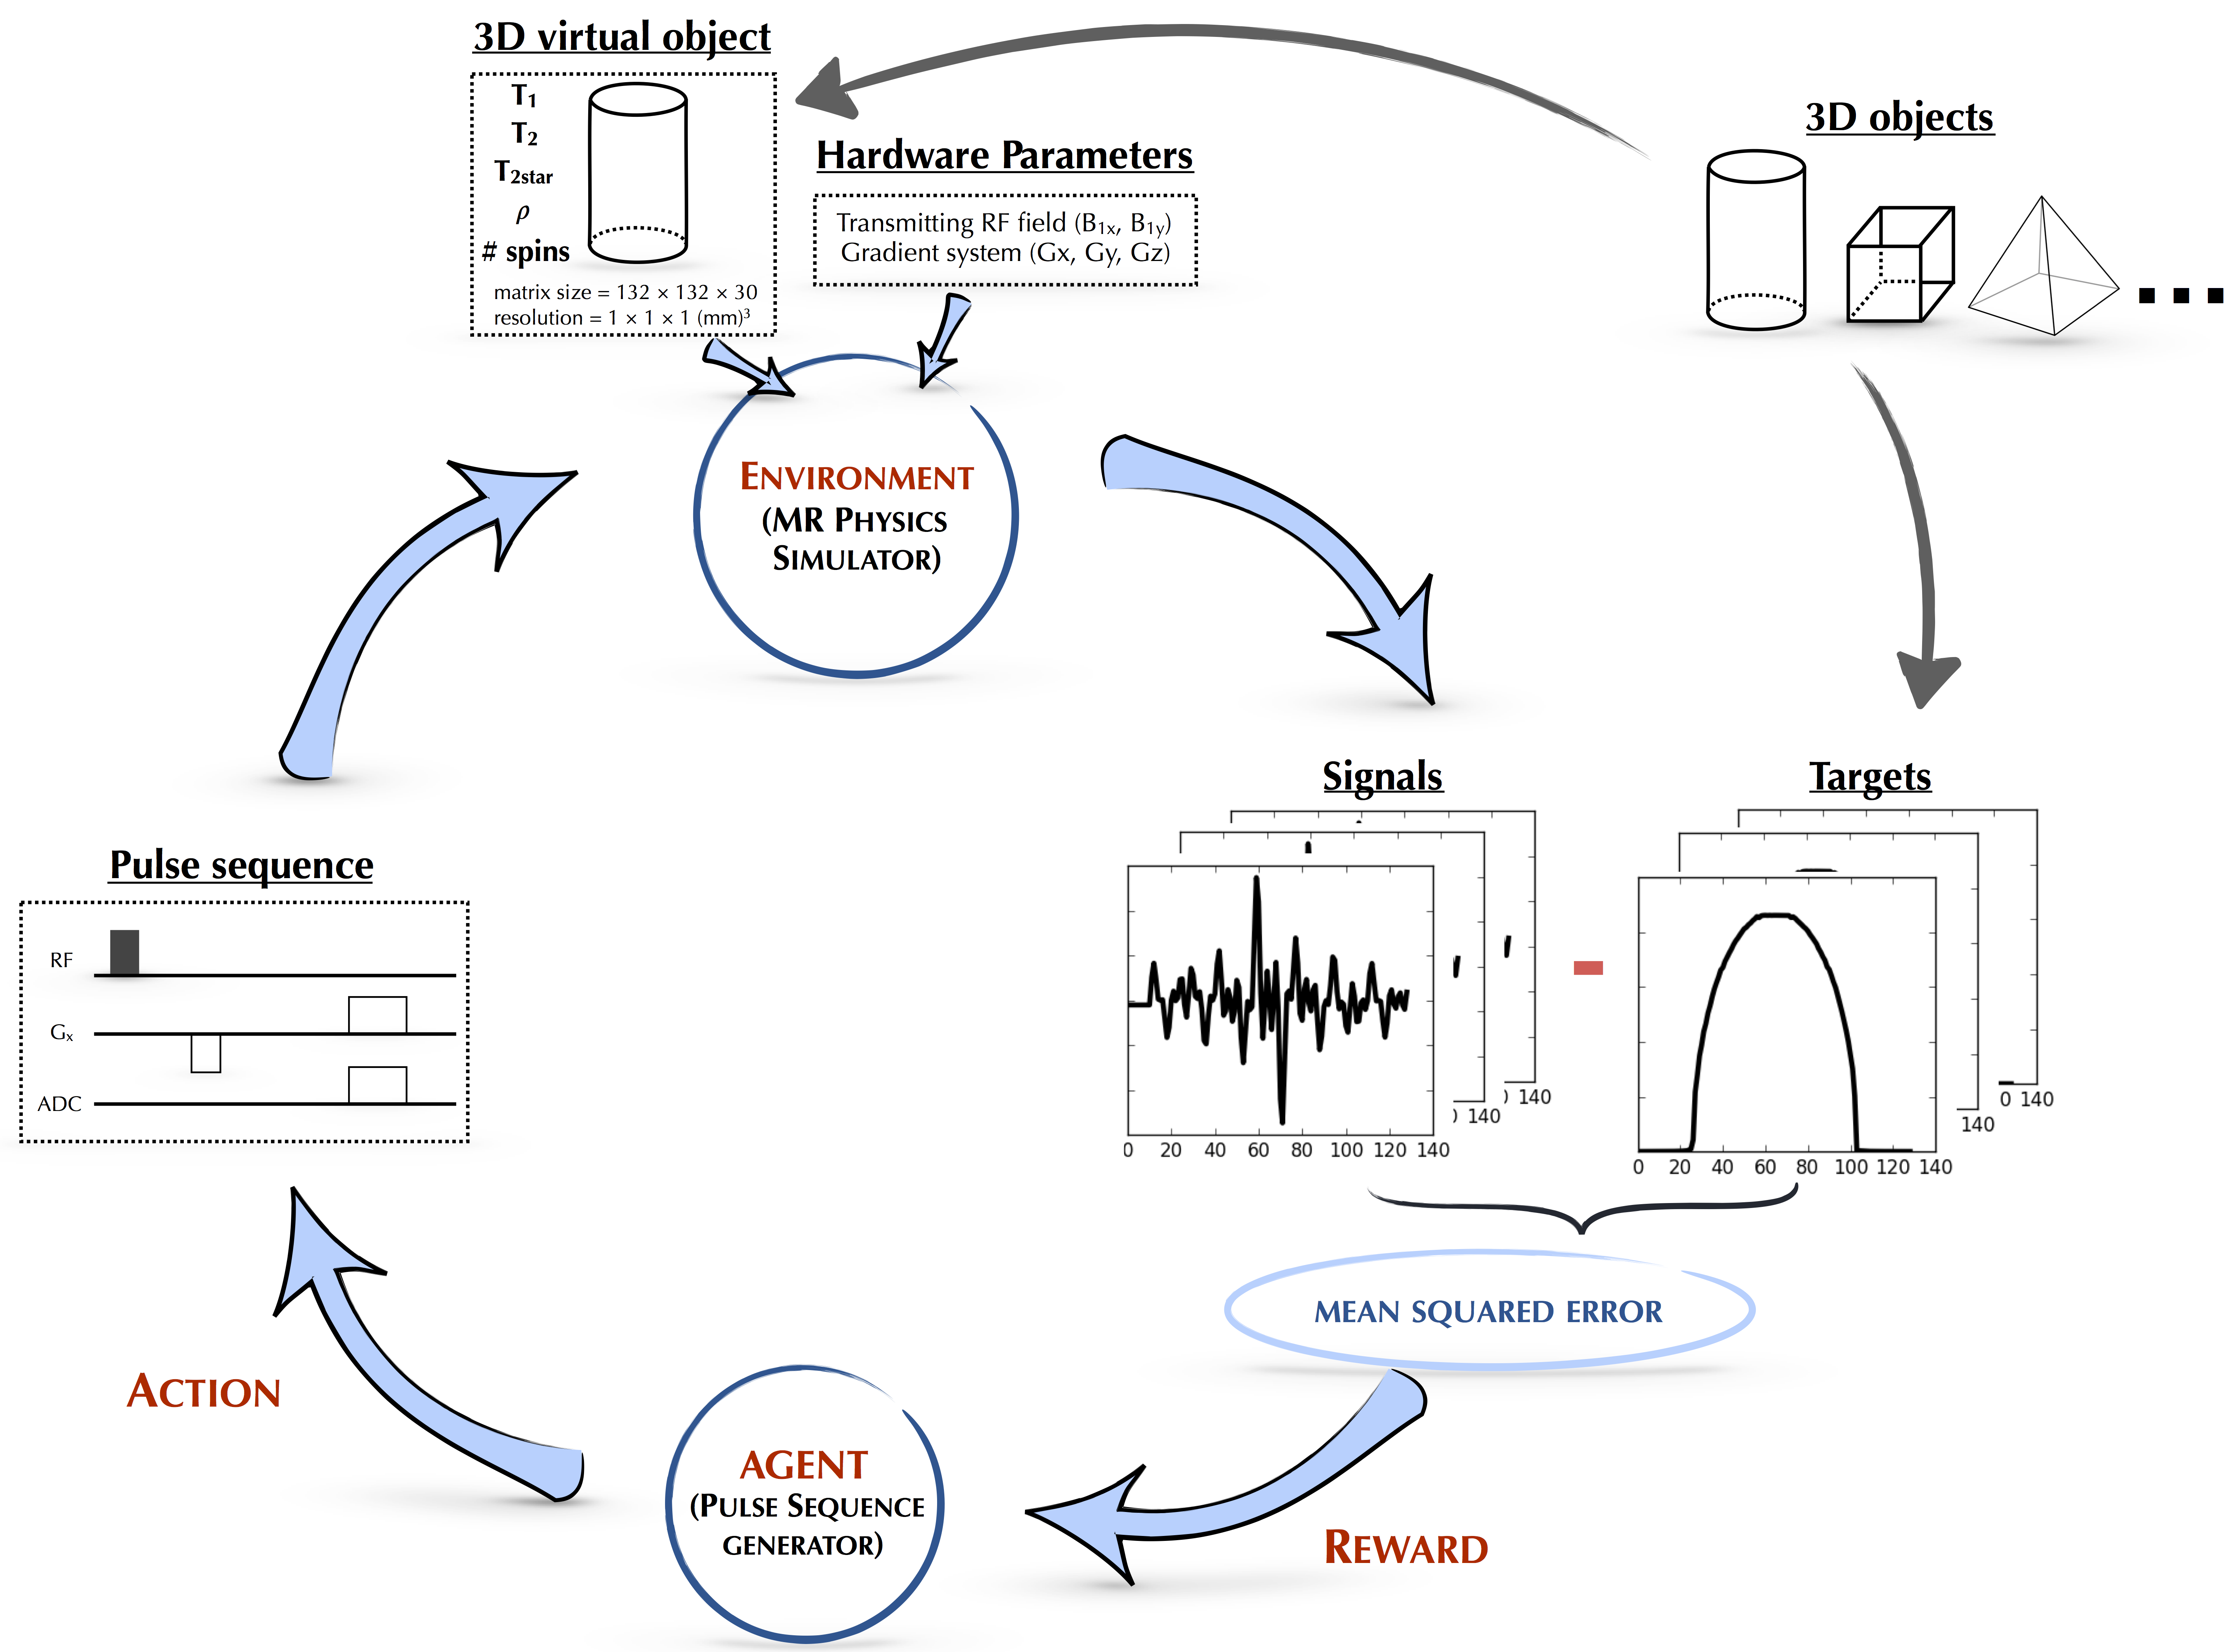
\includegraphics[scale=0.6]{schematic.png}
    \caption{title}
    \label{schematic}
\end{figure}

\section{Challenge}

\section{Reference}
